\chapter{Kode Analisis Regresi Write}
\label{appendix:write-regression-code}

Lampiran ini menunjukkan kode yang digunakan untuk melakukan analisis regresi pada skenario \textit{write} dengan \textit{payload} besar dan \textit{bandwidth} internet menengah. Kode ini bertujuan untuk memperkirakan titik impas antara sistem berbasis \textit{erasure coding} dan sistem berbasis replikasi. Analisis dilakukan dengan menggunakan kakas Jupyter Notebook dan bahasa pemrograman Python, dengan pustaka seperti NumPy, Pandas, Matplotlib, dan Scikit-learn.

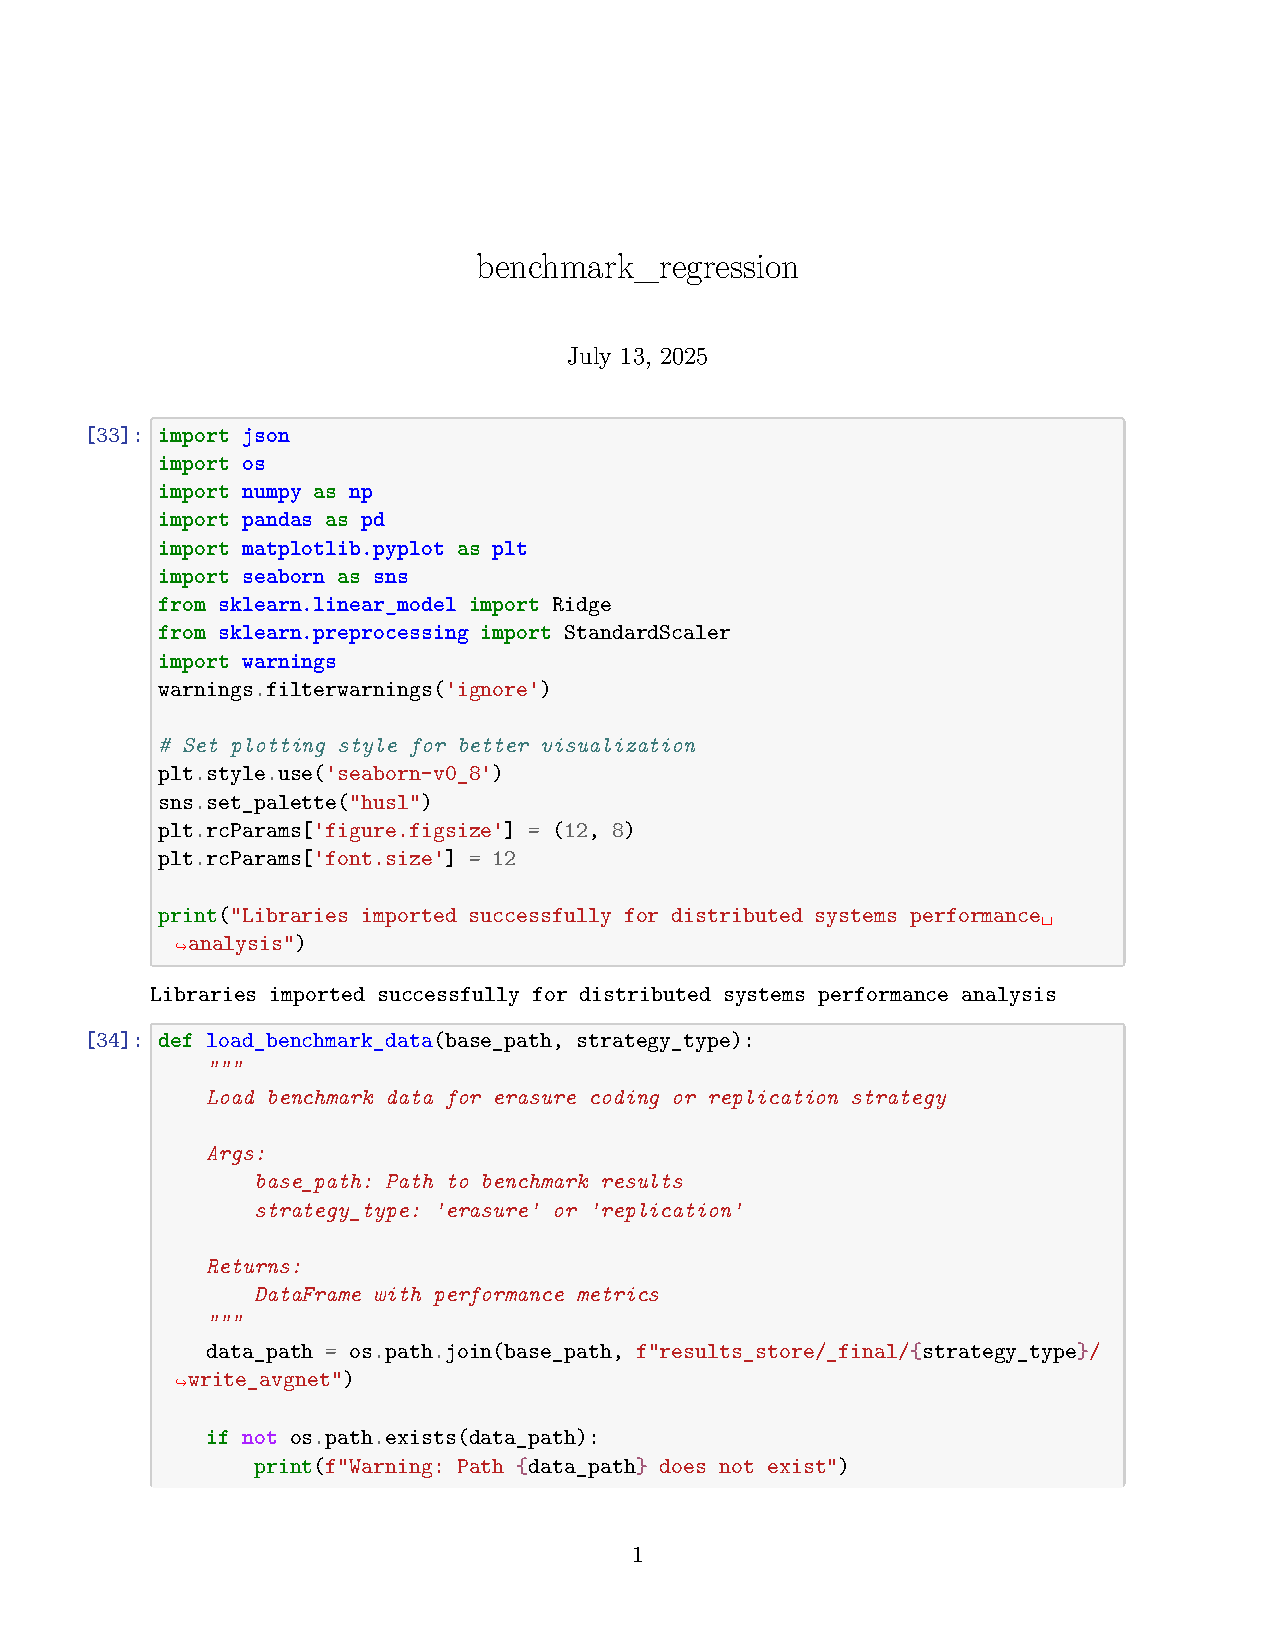
\includepdf[pages=-]{resources/appendix/benchmark_regression_write.pdf}